% Options for packages loaded elsewhere
\PassOptionsToPackage{unicode}{hyperref}
\PassOptionsToPackage{hyphens}{url}
%
\documentclass[
]{article}
\usepackage{lmodern}
\usepackage{amssymb,amsmath}
\usepackage{ifxetex,ifluatex}
\ifnum 0\ifxetex 1\fi\ifluatex 1\fi=0 % if pdftex
  \usepackage[T1]{fontenc}
  \usepackage[utf8]{inputenc}
  \usepackage{textcomp} % provide euro and other symbols
\else % if luatex or xetex
  \usepackage{unicode-math}
  \defaultfontfeatures{Scale=MatchLowercase}
  \defaultfontfeatures[\rmfamily]{Ligatures=TeX,Scale=1}
\fi
% Use upquote if available, for straight quotes in verbatim environments
\IfFileExists{upquote.sty}{\usepackage{upquote}}{}
\IfFileExists{microtype.sty}{% use microtype if available
  \usepackage[]{microtype}
  \UseMicrotypeSet[protrusion]{basicmath} % disable protrusion for tt fonts
}{}
\makeatletter
\@ifundefined{KOMAClassName}{% if non-KOMA class
  \IfFileExists{parskip.sty}{%
    \usepackage{parskip}
  }{% else
    \setlength{\parindent}{0pt}
    \setlength{\parskip}{6pt plus 2pt minus 1pt}}
}{% if KOMA class
  \KOMAoptions{parskip=half}}
\makeatother
\usepackage{xcolor}
\IfFileExists{xurl.sty}{\usepackage{xurl}}{} % add URL line breaks if available
\IfFileExists{bookmark.sty}{\usepackage{bookmark}}{\usepackage{hyperref}}
\hypersetup{
  pdftitle={STAT 33B Workbook 4},
  pdfauthor={Ming Fong (3035619833)},
  hidelinks,
  pdfcreator={LaTeX via pandoc}}
\urlstyle{same} % disable monospaced font for URLs
\usepackage[margin=1in]{geometry}
\usepackage{color}
\usepackage{fancyvrb}
\newcommand{\VerbBar}{|}
\newcommand{\VERB}{\Verb[commandchars=\\\{\}]}
\DefineVerbatimEnvironment{Highlighting}{Verbatim}{commandchars=\\\{\}}
% Add ',fontsize=\small' for more characters per line
\usepackage{framed}
\definecolor{shadecolor}{RGB}{248,248,248}
\newenvironment{Shaded}{\begin{snugshade}}{\end{snugshade}}
\newcommand{\AlertTok}[1]{\textcolor[rgb]{0.94,0.16,0.16}{#1}}
\newcommand{\AnnotationTok}[1]{\textcolor[rgb]{0.56,0.35,0.01}{\textbf{\textit{#1}}}}
\newcommand{\AttributeTok}[1]{\textcolor[rgb]{0.77,0.63,0.00}{#1}}
\newcommand{\BaseNTok}[1]{\textcolor[rgb]{0.00,0.00,0.81}{#1}}
\newcommand{\BuiltInTok}[1]{#1}
\newcommand{\CharTok}[1]{\textcolor[rgb]{0.31,0.60,0.02}{#1}}
\newcommand{\CommentTok}[1]{\textcolor[rgb]{0.56,0.35,0.01}{\textit{#1}}}
\newcommand{\CommentVarTok}[1]{\textcolor[rgb]{0.56,0.35,0.01}{\textbf{\textit{#1}}}}
\newcommand{\ConstantTok}[1]{\textcolor[rgb]{0.00,0.00,0.00}{#1}}
\newcommand{\ControlFlowTok}[1]{\textcolor[rgb]{0.13,0.29,0.53}{\textbf{#1}}}
\newcommand{\DataTypeTok}[1]{\textcolor[rgb]{0.13,0.29,0.53}{#1}}
\newcommand{\DecValTok}[1]{\textcolor[rgb]{0.00,0.00,0.81}{#1}}
\newcommand{\DocumentationTok}[1]{\textcolor[rgb]{0.56,0.35,0.01}{\textbf{\textit{#1}}}}
\newcommand{\ErrorTok}[1]{\textcolor[rgb]{0.64,0.00,0.00}{\textbf{#1}}}
\newcommand{\ExtensionTok}[1]{#1}
\newcommand{\FloatTok}[1]{\textcolor[rgb]{0.00,0.00,0.81}{#1}}
\newcommand{\FunctionTok}[1]{\textcolor[rgb]{0.00,0.00,0.00}{#1}}
\newcommand{\ImportTok}[1]{#1}
\newcommand{\InformationTok}[1]{\textcolor[rgb]{0.56,0.35,0.01}{\textbf{\textit{#1}}}}
\newcommand{\KeywordTok}[1]{\textcolor[rgb]{0.13,0.29,0.53}{\textbf{#1}}}
\newcommand{\NormalTok}[1]{#1}
\newcommand{\OperatorTok}[1]{\textcolor[rgb]{0.81,0.36,0.00}{\textbf{#1}}}
\newcommand{\OtherTok}[1]{\textcolor[rgb]{0.56,0.35,0.01}{#1}}
\newcommand{\PreprocessorTok}[1]{\textcolor[rgb]{0.56,0.35,0.01}{\textit{#1}}}
\newcommand{\RegionMarkerTok}[1]{#1}
\newcommand{\SpecialCharTok}[1]{\textcolor[rgb]{0.00,0.00,0.00}{#1}}
\newcommand{\SpecialStringTok}[1]{\textcolor[rgb]{0.31,0.60,0.02}{#1}}
\newcommand{\StringTok}[1]{\textcolor[rgb]{0.31,0.60,0.02}{#1}}
\newcommand{\VariableTok}[1]{\textcolor[rgb]{0.00,0.00,0.00}{#1}}
\newcommand{\VerbatimStringTok}[1]{\textcolor[rgb]{0.31,0.60,0.02}{#1}}
\newcommand{\WarningTok}[1]{\textcolor[rgb]{0.56,0.35,0.01}{\textbf{\textit{#1}}}}
\usepackage{graphicx}
\makeatletter
\def\maxwidth{\ifdim\Gin@nat@width>\linewidth\linewidth\else\Gin@nat@width\fi}
\def\maxheight{\ifdim\Gin@nat@height>\textheight\textheight\else\Gin@nat@height\fi}
\makeatother
% Scale images if necessary, so that they will not overflow the page
% margins by default, and it is still possible to overwrite the defaults
% using explicit options in \includegraphics[width, height, ...]{}
\setkeys{Gin}{width=\maxwidth,height=\maxheight,keepaspectratio}
% Set default figure placement to htbp
\makeatletter
\def\fps@figure{htbp}
\makeatother
\setlength{\emergencystretch}{3em} % prevent overfull lines
\providecommand{\tightlist}{%
  \setlength{\itemsep}{0pt}\setlength{\parskip}{0pt}}
\setcounter{secnumdepth}{-\maxdimen} % remove section numbering
\ifluatex
  \usepackage{selnolig}  % disable illegal ligatures
\fi

\title{STAT 33B Workbook 4}
\author{Ming Fong (3035619833)}
\date{Sep 24, 2020}

\begin{document}
\maketitle

This workbook is due \textbf{Sep 24, 2020} by 11:59pm PT.

The workbook is organized into sections that correspond to the lecture
videos for the week. Watch a video, then do the corresponding exercises
\emph{before} moving on to the next video.

Workbooks are graded for completeness, so as long as you make a clear
effort to solve each problem, you'll get full credit. That said, make
sure you understand the concepts here, because they're likely to
reappear in homeworks, quizzes, and later lectures.

As you work, write your answers in this notebook. Answer questions with
complete sentences, and put code in code chunks. You can make as many
new code chunks as you like.

In the notebook, you can run the line of code where the cursor is by
pressing \texttt{Ctrl} + \texttt{Enter} on Windows or \texttt{Cmd} +
\texttt{Enter} on Mac OS X. You can run an entire code chunk by clicking
on the green arrow in the upper right corner of the code chunk.

Please do not delete the exercises already in this notebook, because it
may interfere with our grading tools.

You need to submit your work in two places:

\begin{itemize}
\tightlist
\item
  Submit this Rmd file with your edits on bCourses.
\item
  Knit and submit the generated PDF file on Gradescope.
\end{itemize}

\hypertarget{r-graphics-overview}{%
\section{R Graphics Overview}\label{r-graphics-overview}}

Watch the ``R Graphics Overview'' lecture video.

No exercises for this section. Keep at it!

\hypertarget{the-tidyverse}{%
\section{The Tidyverse}\label{the-tidyverse}}

Watch the ``The Tidyverse'' lecture video.

\hypertarget{exercise-1}{%
\subsection{Exercise 1}\label{exercise-1}}

How many packages are in the Tidyverse? Explore the website to find out.
You can count the tidymodels packages as a single package.

YOUR ANSWER GOES HERE:

There are 27 packages in the Tidyverse.

\hypertarget{tibbles}{%
\section{Tibbles}\label{tibbles}}

Watch the ``Tibbles'' lecture video.

\hypertarget{exercise-2}{%
\subsection{Exercise 2}\label{exercise-2}}

Read the documentation for the tibble package on the website.

\begin{enumerate}
\def\labelenumi{\arabic{enumi}.}
\item
  Create a tibble with 4 rows and 3 columns from vectors. You can make
  up the data in the vectors. Use a different data type for each column.
\item
  Show how to convert the tibble to an ordinary data frame.
\end{enumerate}

YOUR ANSWER GOES HERE:

\begin{Shaded}
\begin{Highlighting}[]
\KeywordTok{library}\NormalTok{(tibble)}
\NormalTok{tib =}\StringTok{ }\KeywordTok{tibble}\NormalTok{(}\StringTok{"name"}\NormalTok{ =}\StringTok{ }\KeywordTok{c}\NormalTok{(}\StringTok{"bob"}\NormalTok{, }\StringTok{"joe"}\NormalTok{, }\StringTok{"ted"}\NormalTok{, }\StringTok{"ned"}\NormalTok{),}
   \StringTok{"age"}\NormalTok{ =}\StringTok{ }\DecValTok{4}\OperatorTok{:}\DecValTok{7}\NormalTok{, }\StringTok{"height"}\NormalTok{ =}\StringTok{ }\KeywordTok{c}\NormalTok{(}\FloatTok{8.8}\NormalTok{, }\FloatTok{5.6}\NormalTok{, }\FloatTok{1.5}\NormalTok{, }\FloatTok{0.4}\NormalTok{))}
\NormalTok{tib}
\end{Highlighting}
\end{Shaded}

\begin{verbatim}
## # A tibble: 4 x 3
##   name    age height
##   <chr> <int>  <dbl>
## 1 bob       4    8.8
## 2 joe       5    5.6
## 3 ted       6    1.5
## 4 ned       7    0.4
\end{verbatim}

\begin{Shaded}
\begin{Highlighting}[]
\KeywordTok{as.data.frame}\NormalTok{(tib)}
\end{Highlighting}
\end{Shaded}

\begin{verbatim}
##   name age height
## 1  bob   4    8.8
## 2  joe   5    5.6
## 3  ted   6    1.5
## 4  ned   7    0.4
\end{verbatim}

\hypertarget{the-grammar-of-graphics}{%
\section{The Grammar of Graphics}\label{the-grammar-of-graphics}}

Watch the ``The Grammar of Graphics'' lecture video.

\hypertarget{exercise-3}{%
\subsection{Exercise 3}\label{exercise-3}}

Use ggplot2 and the dogs data to make a scatterplot that shows the
relationship between height and weights. In 2-3 sentences, discuss any
patterns you see in the plot.

YOUR ANSWER GOES HERE:

There is a strong positive correlation between dog height and weight.
The relation appears to be non-linear.

\begin{Shaded}
\begin{Highlighting}[]
\KeywordTok{library}\NormalTok{(ggplot2)}
\NormalTok{dogs =}\StringTok{ }\KeywordTok{readRDS}\NormalTok{(}\StringTok{"C:}\CharTok{\textbackslash{}\textbackslash{}}\StringTok{Users}\CharTok{\textbackslash{}\textbackslash{}}\StringTok{mingf}\CharTok{\textbackslash{}\textbackslash{}}\StringTok{Desktop}\CharTok{\textbackslash{}\textbackslash{}}\StringTok{git}\CharTok{\textbackslash{}\textbackslash{}}\StringTok{STAT33B}\CharTok{\textbackslash{}\textbackslash{}}\StringTok{Week 5}\CharTok{\textbackslash{}\textbackslash{}}\StringTok{data}\CharTok{\textbackslash{}\textbackslash{}}\StringTok{dogs.rds"}\NormalTok{)}
\KeywordTok{ggplot}\NormalTok{(dogs, }\KeywordTok{aes}\NormalTok{(}\DataTypeTok{x =}\NormalTok{ height, }\DataTypeTok{y =}\NormalTok{ weight)) }\OperatorTok{+}\StringTok{ }\KeywordTok{geom\_point}\NormalTok{()}
\end{Highlighting}
\end{Shaded}

\begin{verbatim}
## Warning: Removed 98 rows containing missing values (geom_point).
\end{verbatim}

\includegraphics{workbook04_files/figure-latex/unnamed-chunk-2-1.pdf}

\hypertarget{exercise-4}{%
\subsection{Exercise 4}\label{exercise-4}}

Use ggplot2 and the dogs data to make a histogram of longevity. How long
do most dogs typically live? How spread out is the distribution of
lifespans?

YOUR ANSWER GOES HERE:

The distribution of dog breed longevity appears approximately normal.
The mean is about 11.5 years. The max is about 16 and the min is about
6.

\begin{Shaded}
\begin{Highlighting}[]
\KeywordTok{ggplot}\NormalTok{(dogs, }\KeywordTok{aes}\NormalTok{(}\DataTypeTok{x =}\NormalTok{ longevity)) }\OperatorTok{+}\StringTok{ }\KeywordTok{geom\_histogram}\NormalTok{()}
\end{Highlighting}
\end{Shaded}

\begin{verbatim}
## `stat_bin()` using `bins = 30`. Pick better value with `binwidth`.
\end{verbatim}

\begin{verbatim}
## Warning: Removed 37 rows containing non-finite values (stat_bin).
\end{verbatim}

\includegraphics{workbook04_files/figure-latex/unnamed-chunk-3-1.pdf}

\hypertarget{saving-plots}{%
\section{Saving Plots}\label{saving-plots}}

Watch the ``Saving Plots'' lecture video.

No exercises for this section. Almost done!

\hypertarget{customizing-plots}{%
\section{Customizing Plots}\label{customizing-plots}}

Watch the ``Customizing Plots'' lecture video.

\hypertarget{exercise-5}{%
\subsection{Exercise 5}\label{exercise-5}}

Revisit your scatterplot from Exercise 3. Make the size of each point
correspond to the size of the dog. Make the color of each point
correspond to how good the dog is with kids. Add an appropriate title
and labels.

\emph{Hint: A ``low'' score for kids means the dog is bad with kids.}

YOUR ANSWER GOES HERE:

\begin{Shaded}
\begin{Highlighting}[]
\NormalTok{dogs}\OperatorTok{$}\NormalTok{size =}\StringTok{ }\KeywordTok{factor}\NormalTok{(dogs}\OperatorTok{$}\NormalTok{size, }\DataTypeTok{levels =} \KeywordTok{rev}\NormalTok{(}\KeywordTok{levels}\NormalTok{(dogs}\OperatorTok{$}\NormalTok{size)))}
\KeywordTok{ggplot}\NormalTok{(dogs, }\KeywordTok{aes}\NormalTok{(}\DataTypeTok{x =}\NormalTok{ height, }\DataTypeTok{y =}\NormalTok{ weight)) }\OperatorTok{+}
\StringTok{   }\KeywordTok{geom\_point}\NormalTok{(}\KeywordTok{aes}\NormalTok{(}\DataTypeTok{size =}\NormalTok{ size, }\DataTypeTok{color =}\NormalTok{ kids)) }\OperatorTok{+}
\StringTok{   }\KeywordTok{labs}\NormalTok{(}\DataTypeTok{title =} \StringTok{"Dogs height vs Weight"}\NormalTok{, }\DataTypeTok{x =} \StringTok{"Weight"}\NormalTok{, }\DataTypeTok{y =} \StringTok{"Height"}\NormalTok{)}
\end{Highlighting}
\end{Shaded}

\begin{verbatim}
## Warning: Using size for a discrete variable is not advised.
\end{verbatim}

\begin{verbatim}
## Warning: Removed 98 rows containing missing values (geom_point).
\end{verbatim}

\includegraphics{workbook04_files/figure-latex/unnamed-chunk-4-1.pdf}

\hypertarget{exercise-6}{%
\subsection{Exercise 6}\label{exercise-6}}

Use ggplot2 and the dogs data to answer each of the following questions.

\begin{enumerate}
\def\labelenumi{\arabic{enumi}.}
\item
  Is there a relationship between how long dogs live and how big (in any
  sense) they are?
\item
  Do small dogs tend to be good with kids? If not, does size seem to be
  related to how good dogs are with kids at all?
\item
  Is there a relationship between size and grooming needs?
\end{enumerate}

\emph{Hint: The table from the notes for the next lecture video might
help you decide which plots to use for these questions.}

YOUR ANSWER GOES HERE:

\begin{enumerate}
\def\labelenumi{\arabic{enumi}.}
\tightlist
\item
  There seems to be a weak negative correlation between the longevity
  and weight of dogs. Small dogs tend to live longer than big ones.
\end{enumerate}

\begin{Shaded}
\begin{Highlighting}[]
\KeywordTok{ggplot}\NormalTok{(dogs, }\KeywordTok{aes}\NormalTok{(}\DataTypeTok{x =}\NormalTok{ longevity, }\DataTypeTok{y =}\NormalTok{ weight)) }\OperatorTok{+}
\StringTok{   }\KeywordTok{geom\_point}\NormalTok{() }\OperatorTok{+}
\StringTok{   }\KeywordTok{labs}\NormalTok{(}\DataTypeTok{title =} \StringTok{"Dogs Height vs Longevity"}\NormalTok{, }\DataTypeTok{x =} \StringTok{"Longevity"}\NormalTok{, }\DataTypeTok{y =} \StringTok{"Weight"}\NormalTok{)}
\end{Highlighting}
\end{Shaded}

\begin{verbatim}
## Warning: Removed 99 rows containing missing values (geom_point).
\end{verbatim}

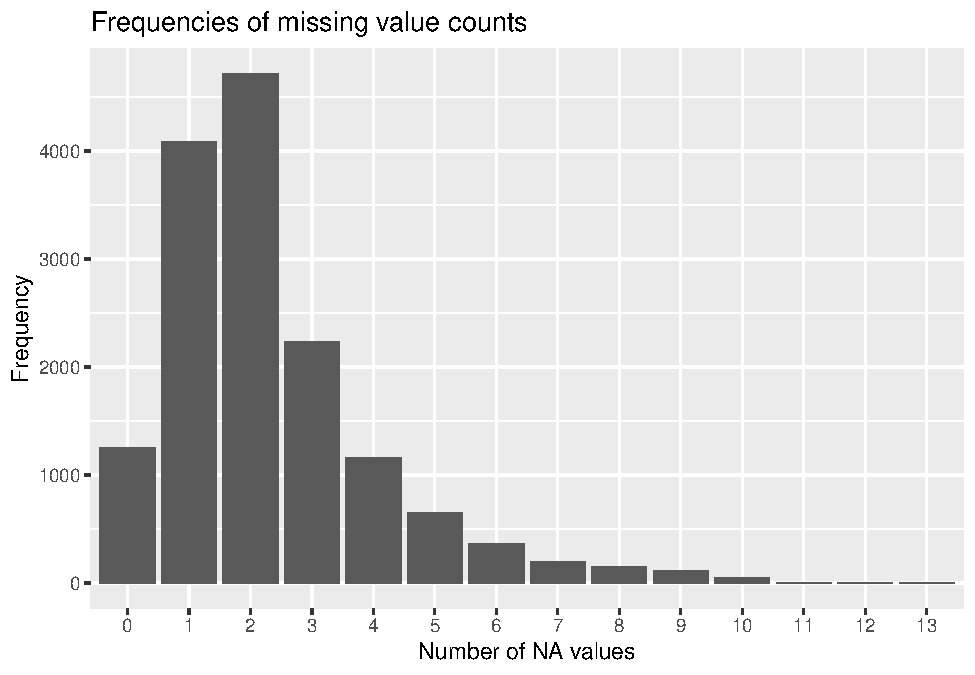
\includegraphics{workbook04_files/figure-latex/unnamed-chunk-5-1.pdf}

\begin{enumerate}
\def\labelenumi{\arabic{enumi}.}
\setcounter{enumi}{1}
\tightlist
\item
  The trend seems to be that the larger the dog, the better it is with
  children.
\end{enumerate}

\begin{Shaded}
\begin{Highlighting}[]
\KeywordTok{ggplot}\NormalTok{(}\DataTypeTok{data =} \KeywordTok{subset}\NormalTok{(dogs, }\OperatorTok{!}\KeywordTok{is.na}\NormalTok{(kids)), }\KeywordTok{aes}\NormalTok{(}\DataTypeTok{fill =}\NormalTok{ kids, }\DataTypeTok{x =}\NormalTok{ size)) }\OperatorTok{+}
\StringTok{   }\KeywordTok{geom\_bar}\NormalTok{(}\DataTypeTok{position =} \StringTok{"fill"}\NormalTok{)}
\end{Highlighting}
\end{Shaded}

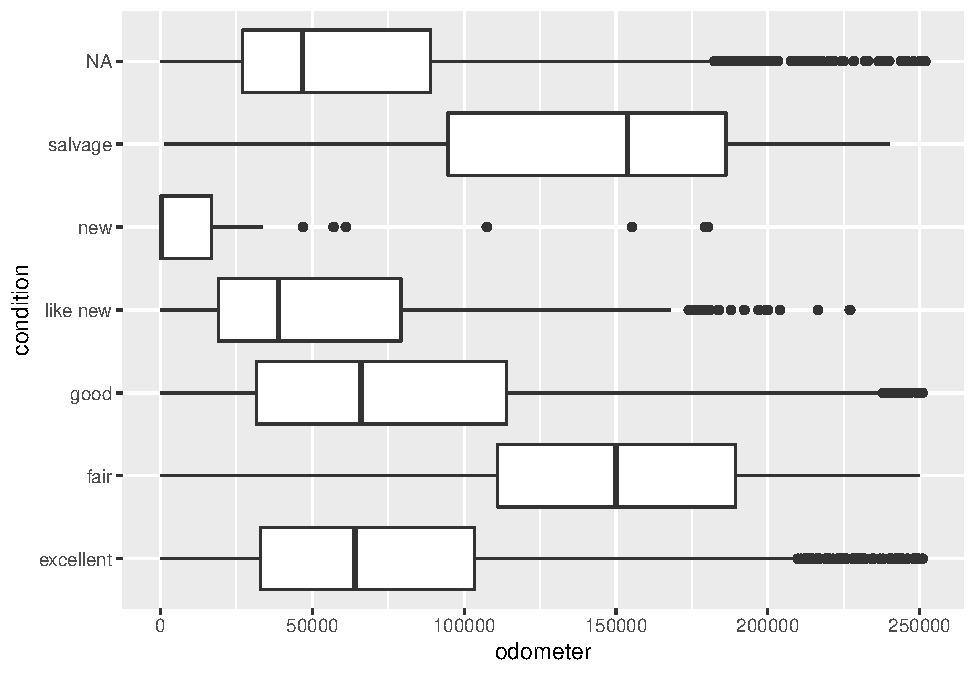
\includegraphics{workbook04_files/figure-latex/unnamed-chunk-6-1.pdf}

\hypertarget{exploratory-data-analysis}{%
\section{Exploratory Data Analysis}\label{exploratory-data-analysis}}

This lecture video is \textbf{OPTIONAL}. You can skip it if you like.

The ``Exploratory Data Analysis'' video discusses how to choose an
appropriate plot for a given set of columns.

No exercises for this section.

\end{document}
